\chapter{Cronograma}
\label{sec:cronograma}
A continuaci\'on se listan las actividades con su estimaci\'on de tiempo:
\begin{itemize}
\item Estudiar \textit{API} de FourSquare: 8 d\'ias
\item Realizar \textit{script} en Python con llamadas de prueba a la \textit{API} de FourSquare: 3 d\'ias
\item Redactar informe \textit{API} FourSquare: 1 d\'ia
\item Estudiar modelos de reconocimiento de patrones: 30 d\'ias
\item Seleccionar el modelo de reconocimiento: 8 d\'ias
\item Redactar informe de modelos de reconocimiento: 2 d\'ias
\item Elecci\'on de perfil de cliente para piloto: 3 d\'ias
\item Estudio de paradigma \textit{MapReduce}: 30 d\'ias
\item Realizaci\'on de ejercicios de aplicaci\'on \textit{MapReduce}: 15 d\'ias
\item Adaptaci\'on de modelo de reconocimiento a \textit{MapReduce}: 30 d\'ias
\item Integraci\'on con API de FourSquare: 20 d\'ias
\item Pruebas preliminares: 5 d\'ias
\item Ajustes necesarios 10 d\'ias
\item Prueba piloto y validaci\'on: 10 d\'ias
\item Escritura de documento de proyecto: 20 d\'ias
\end{itemize}
La figura \ref{fig:dgantt} contiene un diagrama Gantt del cronograma, empezando en marzo primero de 2013:
\begin{figure}[h]
\begin{center}
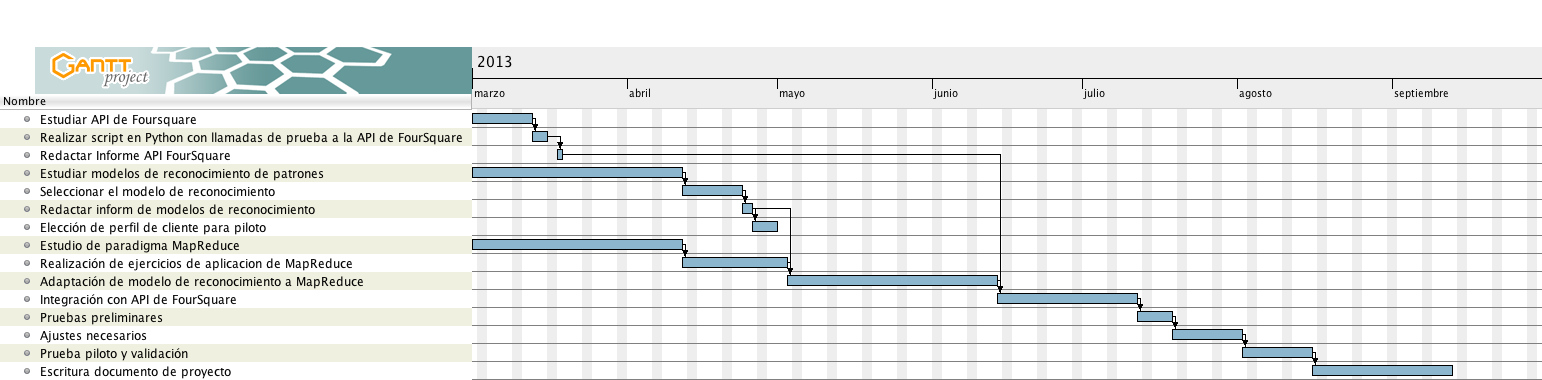
\includegraphics[scale=0.3]{./CronogramaProyectoGrado.png}
\end{center}
{\caption{Diagrama Gantt}\label{fig:dgantt}}
\end{figure}

\pagebreak